\documentclass[aps,prl,twocolumn,superscriptaddress,amsmath,nofootinbib,10pt,floatfix]{revtex4-2}
% \usepackage{graphicx}
% \usepackage[normalem]{ulem}
% \usepackage{xcolor}
% %\usepackage{comment}
% \usepackage{textgreek}
% \usepackage[colorlinks, linkcolor=blue, citecolor=blue]{hyperref}
% \usepackage{gensymb}

% \usepackage{amssymb}

% \documentclass[aps,twocolumn,prl,amsmath,nofootinbib,longbibliography,amssymb,superscriptaddress,10pt]{revtex4-2}
% %twocolumn (removed from \documentclass)

\usepackage[english]{babel}
\usepackage{graphicx}
\usepackage{ulem}
\usepackage{soul}
\usepackage{float} %added by Evyatar
%\usepackage{txfonts}
\usepackage[colorlinks, linkcolor=red , citecolor= blue,breaklinks=true]{hyperref}
%\usepackage{breakurl}
\usepackage{bm}
\usepackage{verbatim}
\usepackage{esint}
\usepackage{marginnote}
\usepackage{feynmf}


\Urlmuskip=0mu plus 1mu

\renewcommand{\vec}[1]{\boldsymbol{#1}}
\newcommand{\RNum}[1]{\uppercase\expandafter{\romannumeral #1\relax}}

\def \k {{\vec k}}
\def \p {{\vec p}}
\def \e {\epsilon}
\def \ve {\varepsilon}
\def \r {{\vec r}}
\def \A {\mathrm{A}}
\def \B {\mathrm{B}}
\def \C {\mathrm{C}}
\def \v {{\bf v}}
\def \el {\ell}
\def \s {\vec{s}}
\def \q {{\vec q}}
\def \d{\partial}
\def \Q{{\cal Q}}
\def \l {\ell}
\def \ve {\varepsilon}
\def \dv {\delta\vec{\varphi}}
\def \S {{\cal{S}}}
\def \G {{\cal{G}}}
\def \C {{\cal{C}}}
\def \K {{\vec K}}
\def \x {{\vec x}}
\def \y {{\vec y}}
\def \Y {\mathbb{Y}}
\def \P {\vec{\Phi}}
\def \Ps {\Psi}
\def \Ph{\Phi}
\def \D{\Delta}
\def \t {\theta}
\def \ol{\overline}
\def \n{{\mathbf{n}}}
\def \L{{\cal{L}}}
\def \O {\cal{O}}
\def \beq {\begin{eqnarray}}
\def \eeq {\end{eqnarray}}
\def \tn {\textnormal}
\def \PP {{\cal {P}}}
\def \M{{\cal {M}}}
\def \Z {{\cal {Z}}}
\def \F {{\cal {F}}}
\def \E {{\cal {E}}}
\def \N {{\cal{N}}}
\def \m {{\mathcal}}
\def \kpa {\kappa_\Vert}
\def \kpe {\kappa_\perp}
\def \ol{\overline}
\def \th{\vartheta}
\def \la{\langle}
\def \ra{\rangle}
\def \ua {\uparrow}
\def \da {\downarrow}
\def \tn {\textnormal}
\def \nn {\nonumber}
%\raggedbottom
\newcommand*{\JFM}[1]{\textcolor{cyan}{ JFM: {#1}}}

\begin{document}


\clearpage
\renewcommand{\thefigure}{S\arabic{figure}}
\renewcommand{\figurename}{Supplemental Figure}
\setcounter{figure}{0}
\appendix
\pagenumbering{arabic}
\begin{widetext}

\begin{center}
  \textbf{\large SUPPLEMENTARY INFORMATION}\\[.2cm]
  \textbf{\large $T-$linear resistivity from magneto-elastic scattering: application to PdCrO$_2$}\\[.2cm]
  %%%%%%
  J.F. Mendez-Valderrama$^{1,*}$, Evyatar Tulipman$^{2,*}$, Elina Zhakina$^{3}$, \\ Andrew P. Mackenzie$^{3,4}$, Erez Berg$^{2}$, and Debanjan Chowdhury$^{1}$
  
  %%%%%%
  {\itshape
        \mbox{$^{1}$Department of Physics, Cornell University, Ithaca, New York 14853, USA.}\\
        \mbox{$^{2}$Department of Condensed Matter Physics, Weizmann Institute of Science, Rehovot 76100, Israel}\\
  	\mbox{$^{3}$Max Planck Institute for Chemical Physics of Solids, N\"othnitzer Stra\ss e 40, 01187 Dresden, Germany}\\
   \mbox{$^{4}$Scottish Universities Physics Alliance, School of Physics \& Astronomy, }
   \mbox{University of St. Andrews, St. Andrews KY16 9SS, United Kingdom}
	
 }
\end{center}
\let\thefootnote\relax\footnote{* These authors contributed equally to this work}


\section{Derivation of the EME coupling} \label{appendix_model}

We derive the low-energy effective Kondo lattice model with EME term starting from an Anderson-type model coupled to phonons; the Kondo term was already derived in Ref.~\cite{sunko_probing_2020}.
The key new insight is as follows: the effective Kondo-like coupling
that is generated between the Pd-electrons and Cr local moments involves
an inter-layer hybridization, $t_{cp,ij}$ between sites $i$ and $j$.
If this coupling were to be affected by the fluctuations associated
with the corresponding out-of-plane bond, $t_{cp,ij}$ will be renormalized
by the displacement, $\varphi^{(O)}_{ij}$. Starting with the microscopic
Hamiltonian,
\begin{align}
H & =H_{\text{Pd}}+H_{\text{Cr}}+H_{\text{hyb}}+H_{\text{ph,EME}},\\
H_{\text{Pd}} & =\sum_{\boldsymbol{k}\sigma}\left(\varepsilon_{\boldsymbol{k}}-\mu\right)p_{\boldsymbol{k}\sigma}^{\dagger}p_{\boldsymbol{k}\sigma},\\
H_{\text{Cr}} & =-\sum_{ij\sigma}t_{ij}^{c}c_{i}^{\dagger}c_{j}+\text{h.c}+U\sum_{i}\left(n_{i\uparrow}^{c}-\frac{1}{2}\right)\left(n_{i\downarrow}^{c}-\frac{1}{2}\right),\\
H_{\text{hyb}} & =\sum_{\left\langle ij\right\rangle \sigma}t_{cp,ij}\left(1-\eta\varphi^{(O)}_{ij}\right)\left(c_{i\sigma}^{\dagger}p_{j\sigma}+\text{h.c}\right)\\
H_{\text{ph,EME}} & =\sum_{\left\langle ij\right\rangle }\frac{\pi_{ij}^{(O)\,2}}{2M}+\frac{M\tilde{\omega}_{0}}{2}\varphi_{ij}^{(O)\,2},
\end{align}
where $c,~c^\dagger$ represent the Cr-electron operators, $t_{ij}^{c}$ is a nearest-neighbor hopping in the Cr layer, $\varepsilon_{\boldsymbol{k}}$
is the dispersion for the Pd electrons, $\eta$ determines the scale by which
the hybridization is renormalized to leading order in the bond displacement
$\varphi^{(O)}_{ij}$, $M$ is the phonon mass, $n_{i\sigma}^{c}$ is the
density operator for Cr electrons, and $U$ is the on site interaction
strength. In general, these interactions  involve multiple orbitals associated with the Cr crystal field multiplets, and contain the full lattice structure of PdCrO$_{2}$. However, here for simplicity, we only retain a single orbital per site in the Cr layers.

We consider the strong-coupling limit, $U\gg t^{c},g$ (similarly to Ref.~\cite{sunko_probing_2020}), and derive the low-energy model based on a Schriffer-Wolff transformation. Retaining terms up to linear-order in the bond displacement, we obtain:
\begin{align}
H & =H_{\text{Pd}}+H_{\text{lm}}+H_{\text{K}}+H_{\text{EME}}+H_{\text{ph,EME}},\\
H_{\text{lm}} & =J_{H}\sum_{\left\langle ij\right\rangle }\boldsymbol{S}_{i}\cdot\boldsymbol{S}_{j}\\
H_{\text{K}} & =\sum_{\left\langle ilj\right\rangle \sigma}\frac{4t_{cp,ij}t_{cp,lj}}{U}\boldsymbol{S}_{l}\cdot\left(p_{i}^{\dagger}\boldsymbol{\sigma}p_{j}\right)\\
H_{\text{EME}} & =-\sum_{\left\langle ilj\right\rangle \sigma}\frac{4t_{cp,ij}t_{cp,lj}}{U}\eta\left(\varphi^{(O)}_{il}+\varphi^{(O)}_{jl}\right)\boldsymbol{S}_{l}\cdot\left(p_{i}^{\dagger}\boldsymbol{\sigma}p_{j}\right)
\end{align}

The first term above is the usual Heisenberg coupling with antiferromagnetic
exchange $J_{H}=4(t^{c})^2/U$. The second term  is a Kondo coupling \cite{sunko_probing_2020} with the appropriate form-factors coming from the fact that the interaction is inter-layer. The third term is the new EME coupling
between local moments in the Cr layer, optical phonons and itinerant Pd-electrons. In what follows, we consider the simplified case where the adjacent Pd layers are stacked in a perfectly aligned arrangement, and the hybridization is independent of the bond direction, i.e. $t_{cp,ij}\rightarrow t_{cp}$. In
this limit, we can define the Kondo and EME couplings to be $J_{K}=4t_{cp}^{2}/U$
and $\tilde{\alpha}=-J_{K}\eta$. We then have the following Hamiltonian
in momentum space
\begin{equation}
H=H_{\text{Pd}}+H_{\text{ph}}+H_{\text{lm}}+H_{\text{int}}
\end{equation}

with the interaction given by
\begin{align}
H_{\text{int}}= & \frac{1}{\sqrt{N}}\sum_{\substack{\bm{k}\bm{k}'\\
\alpha\beta
}
}J_{K}\left(\boldsymbol{k},\boldsymbol{k}'\right)p_{\boldsymbol{k}\alpha}^{\dagger}\left[\boldsymbol{S}_{\boldsymbol{k}-\boldsymbol{k}'}\cdot\boldsymbol{\sigma}_{\alpha\beta}\right]p_{\boldsymbol{k}'\beta}\\
 & +\frac{1}{N}\sum_{\bm{k}\bm{k}'\bm{q}}\sum_{\ell\alpha\beta}\tilde{\alpha}_{\ell}\left(\boldsymbol{k},\boldsymbol{k}'\right)\varphi^{(O)}_{\ell}\left(\boldsymbol{k}-\boldsymbol{k}'-\boldsymbol{q}\right)p_{\boldsymbol{k}\alpha}^{\dagger}\left[\boldsymbol{S}_{\boldsymbol{q}}\cdot\boldsymbol{\sigma}_{\alpha\beta}\right]p_{\boldsymbol{k}'\beta}
\end{align}

where the Fourier transformed operators are:
\begin{equation}
\varphi^{(O)}_{\ell+j,j}=\frac{1}{\sqrt{N}}\sum_{\bm{k}}e^{-i\bm{k}\bm{R}_{j}}\varphi^{(O)}_{\ell}\left(\boldsymbol{k}\right)
\end{equation}

\begin{equation}
p_{i\alpha}^{\dagger}=\frac{1}{\sqrt{N}}\sum_{\bm{k}}e^{-i\bm{k}\bm{R}_{i}}p_{\boldsymbol{k}\alpha}^{\dagger}
\end{equation}
\begin{equation}
\boldsymbol{S}_{j}=\frac{1}{\sqrt{N}}\sum_{\bm{q}}e^{-i\bm{q}\bm{R}_{j}}\boldsymbol{S}_{\boldsymbol{q}}
\end{equation}

and the momentum-dependent couplings are 
\begin{align*}
J_{K}\left(\boldsymbol{k},\boldsymbol{k}'\right) & =J_{K}\left[2\cos\left(k_{z}a_{z}\right)\right]\left[2\cos\left(k_{z}'a_{z}\right)\right]\\
\tilde{\alpha}_{+1}\left(\boldsymbol{k},\boldsymbol{k}'\right) & =\tilde{\alpha}_{-1}\left(\boldsymbol{k},\boldsymbol{k}'\right)=\tilde{\alpha}\left(\boldsymbol{k},\boldsymbol{k}'\right)=-\eta J_{K}\left(\boldsymbol{k},\boldsymbol{k}'\right),
\end{align*}
with $\bm{R}_{i}$ being the position of site $i$ and $N$ the number
of unit cells. 

We have introduced three new parameters: the mass of the out-of-plane mode $M$ (appearing in the EME term), its frequency
$\tilde{\omega}_{0}$ and the EME coupling $\eta$. As we detail
in the text, these parameters only enter the theory either in the
precise combination that corresponds to the dimensionless EME coupling,
or in the combination $\beta\tilde{\omega}_{0}$, leaving effectively
two new parameters in the theory. The rest of the parameters are taken
from the values provided in \cite{sunko_probing_2020}. Specifically, we have $U=4$eV
and $t_{cp}=107$meV which lead to a Kondo coupling of $J_{K}=11.45$ meV.
Additionally, we have $J_{H}=6.25$meV, $t_{nn}^{p}=568$meV, $t_{nnn}^{p}=108$meV,
and $\mu=256$meV. We fit the difference
of the resistivity of PdCrO$_{2}$ and PdCoO$_{2}$ to obtain the
dimensionless EME coupling in the main text and the frequency of this mode. 

\section{Transport rate} \label{transport_rate}

Within the variational Boltzmann approach \cite{Ziman_2001} 
the transport
lifetime can estimated by 
\begin{equation}
\rho\leq\frac{\frac{V}{2k_BT}\sum_{\boldsymbol{q}\boldsymbol{p}}P_{\boldsymbol{p}\boldsymbol{q}}\left(\psi_{\boldsymbol{q}}-\psi_{\boldsymbol{p}}\right)^{2}}{\left|\sum_{\boldsymbol{q}}e\frac{\partial f}{\partial\epsilon_{\boldsymbol{q}}}\psi_{\boldsymbol{q}}\boldsymbol{v}\left(\boldsymbol{q}\right)\cdot\boldsymbol{n}\right|^{2}}
\end{equation}
with $\psi_{\boldsymbol{q}}$ a variational anzatz, $P_{\boldsymbol{p}\boldsymbol{q}}$
the transition probaility from different momentum states, $V$ the
volume, $\boldsymbol{n}$ is a unit vector in the direction of the electric field $\boldsymbol{E}$,
$f$ the Fermi-Dirac distribution, $e$ the electron charge, $\boldsymbol{v}\left(\boldsymbol{q}\right)=\partial_{\boldsymbol{q}}\epsilon_{\boldsymbol{q}},$
and $\epsilon_{\boldsymbol{q}}$ the dispersion. Using the ansatz
$\psi_{\boldsymbol{q}}=-e\boldsymbol{v}_{\boldsymbol{q}}\cdot\boldsymbol{E}\tau_{\text{tr}}$
we recover the drude formula with the momentum relaxation time
\begin{equation}
\tau_{\text{tr}}^{-1}=\frac{\frac{1}{k_BT}\sum_{\boldsymbol{q}\boldsymbol{p}}P_{\boldsymbol{p}\boldsymbol{q}}\left(\boldsymbol{v}\left(\boldsymbol{q}\right)\cdot\boldsymbol{n}-\boldsymbol{v}\left(\boldsymbol{q}\right)\cdot\boldsymbol{n}\right)^{2}}{\sum_{\boldsymbol{q}}2\left(-\frac{\partial f}{\partial\epsilon_{\boldsymbol{q}}}\right)\left(\boldsymbol{v}\left(\boldsymbol{q}\right)\cdot\boldsymbol{n}\right)^{2}}.
\label{tr_time_SI}   
\end{equation}

At intermediate-$T$, where the scattering mechanisms are essentially isotropic, Mathiessen's rule is obeyed such that 
\begin{equation}
\tau_{\text{tr}}^{-1}=\tau_{\text{K}}^{-1}+\tau_{\text{EME}}^{-1}+\tau_{\text{el--ph}}^{-1}
\end{equation}
where each individual scattering rate is determined by the transition
probabilities 
\begin{equation}
P_{\boldsymbol{p}\boldsymbol{q}}^{\rm{K}}=k_BT\frac{2\pi}{\hbar}\left(-\frac{\partial f_{\boldsymbol{p}}}{\partial\epsilon_{\boldsymbol{p}}}\right)\left|J_{K}\left(\boldsymbol{p},\boldsymbol{q}\right)\right|^{2}\chi''\left(\boldsymbol{p}-\boldsymbol{q},\varepsilon_{\boldsymbol{p}}-\epsilon_{\boldsymbol{q}}\right)\left(n_{B}\left(\varepsilon_{\boldsymbol{p}}-\epsilon_{\boldsymbol{q}}\right)+n_{F}\left(-\epsilon_{\boldsymbol{q}}\right)\right),
\end{equation}

\begin{align}
P_{\boldsymbol{k}\boldsymbol{p}}^{\rm{EME}} =k_BT\frac{2\pi}{\hbar}\left(-\frac{\partial f}{\partial\epsilon_{\boldsymbol{p}}}\right)\left|\tilde{\alpha}\left(\boldsymbol{p},\boldsymbol{q}\right)\right|^{2} & \sum_{\boldsymbol{k}}\int\frac{d\nu}{\pi}\chi''\left(\boldsymbol{k}+\boldsymbol{p}-\boldsymbol{q},\epsilon_{\boldsymbol{p}}-\nu\right)\mathcal{B}\left(\boldsymbol{k},\nu-\varepsilon_{\boldsymbol{q}}\right) \times \nonumber \\ &\left[n_{B}\left(\epsilon_{\boldsymbol{p}}-\nu\right)+n_{F}\left(-\nu\right)\right]\left[n_{B}\left(\nu-\varepsilon_{\boldsymbol{q}}\right)+n_{F}\left(-\varepsilon_{\boldsymbol{q}}\right)\right],
\end{align}

\begin{equation}
P_{\boldsymbol{p}\boldsymbol{q}}^{\rm{el-ph}}=kT\frac{2\pi}{\hbar}\left(-\frac{\partial f_{\boldsymbol{p}}}{\partial\epsilon_{\boldsymbol{p}}}\right)\sum_{\lambda}\left|\alpha_{\lambda}\left(\boldsymbol{p},\boldsymbol{q}\right)\right|^{2}\mathcal{B}_{\lambda}\left(\boldsymbol{p}-\boldsymbol{q},\varepsilon_{\boldsymbol{p}}-\epsilon_{\boldsymbol{q}}\right)\left(n_{B}\left(\varepsilon_{\boldsymbol{p}}-\epsilon_{\boldsymbol{q}}\right)+f\left(-\epsilon_{\boldsymbol{q}}\right)\right).
\end{equation}
Here $\chi''\left(\boldsymbol{p},\omega\right)$ is the spin susceptibility
and $\mathcal{B}_{\lambda}\left(\boldsymbol{k},\nu\right)$ is the
phonon spectral function for mode $\lambda=o,a$ which can be either
acoustic or optical. We also reintroduced the momentum dependence
in all the couplings. In the case where the magnetic and itinerant
electron layers are perfectly aligned we have 
\begin{equation}
J_{K}\left(\boldsymbol{p},\boldsymbol{q}\right)=J_{K}\left[2\cos\left(p_{z}a_{z}\right)\right]\left[2\cos\left(q_{z}a_{z}\right)\right],
\end{equation}

\begin{equation}
\tilde{\alpha}\left(\boldsymbol{p},\boldsymbol{q}\right)=\tilde{\alpha}\left[2\cos\left(p_{z}a_{z}\right)\right]\left[2\cos\left(q_{z}a_{z}\right)\right],
\end{equation}

\begin{equation}
\alpha_{\rm{o}}\left(\boldsymbol{p},\boldsymbol{q}\right)=\alpha_{\rm{o}},
\end{equation}

and 

\begin{equation}
\alpha_{\rm{a}}\left(\boldsymbol{p},\boldsymbol{q}\right)=\alpha_{\rm{a}}\left|\boldsymbol{p}-\boldsymbol{q}\right|.
\end{equation}
Here the coupling constants are as defined in the main text. Additionally,
we make the local approximation for the spins \cite{mcroberts2022intermediatescale}:
\begin{equation}
\chi''\left(\nu\right)=S\left(S+1\right)\beta\nu\frac{\theta\left(2\pi J_{H}-\left|\nu\right|\right)}{2J_{H}}
\end{equation}
with the sum rule constraint 
\begin{equation}
\int\frac{\chi''\left(\nu\right)}{\beta\nu}d\nu=2\pi S\left(S+1\right).
\end{equation}
The spectral function for the free phonons is given by 
\begin{equation}
\mathcal{B}_{\lambda}\left(\boldsymbol{k},\nu\right)=\frac{\pi\hbar}{2M\omega_{\boldsymbol{k},\lambda}}\left(\delta\left(\nu-\omega_{\boldsymbol{k},\lambda}\right)-\delta\left(\nu+\omega_{\boldsymbol{k},\lambda}\right)\right)
\end{equation}
where for optical phonons we have $\omega_{\boldsymbol{k},o}=\omega_{0}$
while for acoustic phonons $\omega_{\boldsymbol{k},a}=ck$. The integrals
above can then be evaluated analytically if we take a quasi-2D circular
fermi surface. This leads to the total scattering rate: 
\begin{align}
\tau_{\rm{tr}}^{-1} & =2\pi\frac{\lambda_{tr,\rm{EP},o}}{\hbar\beta}\mathcal{I}_{1}\left(\frac{\beta\hbar\omega_{0}}{2}\right)+2\pi\frac{\lambda_{tr,\rm{EP},a}}{\hbar\beta}\mathcal{I}_{2}\left(\frac{\beta\hbar\omega_{BG}}{2}\right) \nonumber\\
 & +2\pi\frac{\lambda_{K}J_{\rm{K}}}{\hbar}\mathcal{I}_{3}\left(2\pi\beta J_{\rm{H}}\right)+2\pi\frac{\lambda_{tr,\rm{EME}}}{\hbar\beta}\mathcal{I}_{4}\left(2\pi\beta J_{\rm{H}},\beta\hbar\tilde{\omega}_{0}\right)
 \label{eqn:transport_rate}
\end{align}

Here we define
\begin{equation}
\mathcal{I}_{1}\left(x\right)=\left[x\text{csch}\left(x\right)\right]^{2},
\label{def_of_K}
\end{equation}
and
\begin{equation}
\mathcal{I}_{2}\left(x\right)=\frac{4}{\pi}\frac{1}{x^{3}}\int_{0}^{x}dy\ \frac{y^{4}}{\sqrt{1-\left(\frac{y}{x}\right)^{2}}}\left[\text{csch}\left(y\right)\right]^{2},
\end{equation}
corresponding to the case of acoustic phonons
interacting with a circular
Fermi surface in two dimensions. In addition,
\begin{align}
\mathcal{I}_{3}\left(y\right) & =-\frac{4\text{Li}_{2}\left(e^{-y}\right)}{y}-\frac{2y}{e^{y}-1}-4y+\frac{2\pi^{2}}{3y}+4\log\left(e^{y}-1\right),
\end{align}
corresponds to the pure Kondo scattering at high temperatures, where the logarithmic integrals result from integrating the Fermi function.
And finally 
\begin{equation}
\mathcal{I}_{4}\left(y,z\right)=\frac{z^{2}}{\cosh\left(z\right)-1}\mathcal{J}\left(y,z\right)
\end{equation}
is the result of the integrals involving the EME coupling, with the
additional definition:
\begin{align}
\mathcal{J}\left(y,z\right) & =\frac{-2z\text{Li}_{2}\left(e^{-y}\right)+\left(2y+z\right)\text{Li}_{2}\left(e^{-y-z}\right)+\left(z-2y\right)\text{Li}_{2}\left(e^{z-y}\right)+2\text{Li}_{3}\left(e^{-y-z}\right)-2\text{Li}_{3}\left(e^{z-y}\right)}{2yz} \nonumber \\
 & +\frac{z^{2}}{12y}-\frac{1}{2}\log\left(\left(e^{y}-e^{z}\right)\left(e^{y+z}-1\right)\right)+\frac{y\log\left(\sinh\left(\frac{y-z}{2}\right)\text{csch}\left(\frac{y+z}{2}\right)\right)}{2z}+\frac{y}{2}+\frac{\pi^{2}}{3y}+\log\left(e^{y}-1\right)+\frac{z}{2}.
\end{align}

These functions have the following high temperature limits which can
be obtained from the asymptotic expansions for the polylogarithm
\begin{equation}
\lim_{T\rightarrow\infty}\mathcal{I}_{1}\left(\frac{\beta\hbar\omega_{0}}{2}\right)=\lim_{T\rightarrow\infty}\mathcal{I}_{2}\left(\frac{\beta\hbar\omega_{BG}}{2}\right)=1
\end{equation}

and 
\begin{equation}
\lim_{T\rightarrow\infty}\mathcal{I}_{3}\left(2\pi\beta J_{H}\right)=\lim_{T\rightarrow\infty}\mathcal{I}_{4}\left(2\pi\beta J_{H},\beta\hbar\tilde{\omega}_{0}\right)=2.
\end{equation}

In the main text, we use the effective mass of PdCoO$_{2}$ extracted
from quantum oscillations given in Ref.~\cite{sunko_angle_2019}, and the density corresponding
to half filling to extract the transport rate from experiments following
the procedure in Ref.~\cite{bruin_similarity_2013} to calculate the ratio $n/m$ for both PdCoO$_{2}$ and PdCrO$_{2}$. Then we fit the resulting scattering
rate to the first two terms which correspond to electron-phonon scattering
in $\tau_{tr}^{-1}$. With this procedure, we find the parameters
$\lambda_{\rm el-ph,o}=0.024$,$\hbar\omega_{0}=120$meV,$\lambda_{\rm el-ph,a}=0.043$,
and $\hbar\omega_{\rm BG}=29$meV, which are in close agreement with the
reported values in \cite{Hicks_mobility_2012, roles_highfreq_pdcoo2_takatsu_2007}. The difference between our treatment
and that in Refs.~\cite{Hicks_mobility_2012, roles_highfreq_pdcoo2_takatsu_2007} is that we consider a 2D fermi surface instead
of a 3D Fermi surface. At intermediate temperatures
where our theory is valid we do not see significant differences in
the fit quality between the model considered here and the ones in
\cite{Hicks_mobility_2012, roles_highfreq_pdcoo2_takatsu_2007} .

We then carry out the same procedure for PdCrO$_{2}$ and substract
the resulting scattering rate from the scattering rate extracted from
PdCoO$_{2}$. This would isolate the last two terms that correspond
to Kondo and EME scattering in $\tau_{tr}^{-1}$. By fitting this
excess scattering rate we find the EME parameters $\lambda_{\rm EME}=0.025$
and $\hbar\tilde{\omega}_{0}=45$meV. Since we use the high temperature
approximation for $\chi''$ we do not fit the low temperature regime
of $\Delta_{\tau}=\tau_{\rm{tr,Cr}}^{-1}-\tau_{\rm{tr,Co}}^{-1}$ but only carry
the fit at temperatures above 80K ($J_{H}\sim72K$). Note that the
constant offset between the PdCoO$_{2}$ and the PdCrO$_{2}$ resistivities
is not fitted. This excess scattering rate comes purely from the Kondo
scattering with the dimensionless coupling $\lambda_{K}=4S\left(S+1\right)J_{K}\nu_{0}$
and a saturation scale set by $J_{H}$, where the value of these couplings
is listed above. 

In the above, one can trace the variuous features of $\rho$ for PdCrO$_{2}$
to each of the terms in Eqn.~\ref{eqn:transport_rate}.The Kondo term increases sharply
and completely saturates at a temperature scale set by $2\pi J_{H}$.
This approach to saturation would be responsible for the sublinear
approach to the $T$--linear regime. This sublinear piece dominates
at $T\sim J_{H}$ over the contributions from the phonon and the magnetoelastic
scattering rates. Eventually, both of these contributions catch up
with the Kondo scattering rate and the resistivity becomes $T$--linear
which can be seen from the high temperature limits of $\mathcal{I}_{4}$
and $\mathcal{I}_{3}$ and the expression for $\tau_{tr}^{-1}$. Taking
the high temperature limit, we can determine the coefficient of the
linear in $T$ scattering rate. Using the asymptotic expressions above
and the values of the fitted dimensionless couplings we get 
\begin{align}
\lim_{T\rightarrow\infty}\frac{d}{dT}\tau_{\rm{tr}}^{-1} & =\left(\frac{k_{B}}{\hbar}\right)2\pi\left(\lambda_{\rm el-ph,o}+\lambda_{\rm el-ph,a}+2\lambda_{\rm EME}\right)\\
 & \sim0.75\left(\frac{k_{B}}{\hbar}\right)
\end{align}
which is close to the Planckian slope $k_B/\hbar$.  

\begin{figure}[h]
\centering
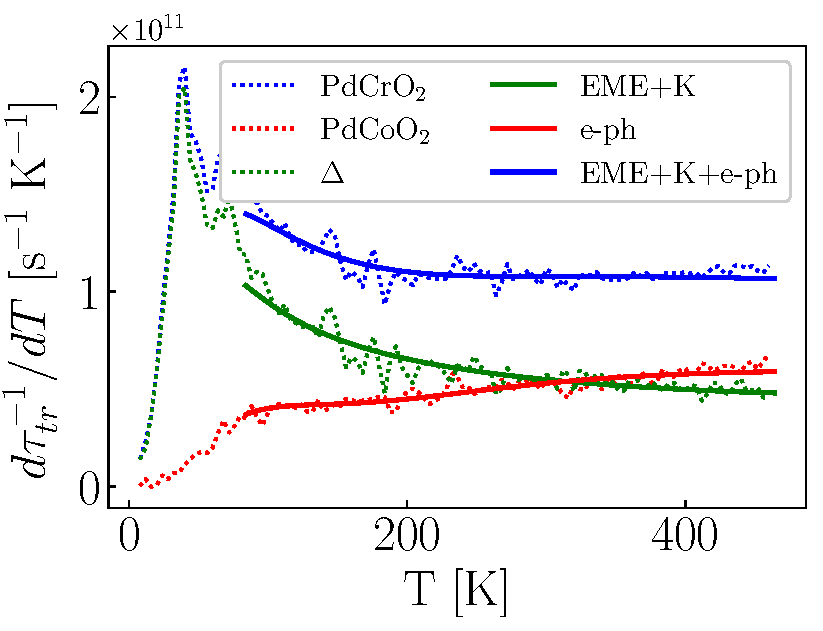
\includegraphics[width=0.45\textwidth]{linear_cr.pdf} 
\caption{Rate of change of the scattering rates from fit and experiments. In the case where the resistivity is completely saturated we expect this quantity to be constant. However, neither the electron-phonon contribution, nor the Kondo and EME contributions are linear. Nevertheless, the sum of the scattering rates is almost linear, as evidenced by the constant rate of change. }
\label{fig:gammatroverT}
\end{figure}

Finally, we note that neither $\tau_{\rm el-ph}^{-1}$ nor $\tau_{\rm K}^{-1}$ are in the fully saturated regime for the values of the fit parameters
obtained from the above procedure (see Fig.~\ref{fig:gammatroverT}). In contrast, the excess resistivity from the EME
term is generated by a mode that saturates at relatively low temperatures (since the out-of-plane vibration in PdCrO$_2$ turns out to be softer than the in-plane one). At the same time, the addition of the pure Kondo scattering gives
an additional $T$-sublinear contribution to the resistivity. In
total, the $T$-superlinear scattering rate from electron-phonon scattering
and the $T$-sublinear contribution from the Kondo term, together with the $T$-linear EME contribution yield an approximately $T$--linear resistivity for PdCrO$_{2}$.


\section{Out-of-plane resistivity} \label{appendix_caxis}


The starting point of our discussion is a slightly modified version of the model introduced in the discussion of in-plane transport. Here, we assume that in addition to the regular in-plane hopping in the Pd layer, we have a small but non negligible hopping $t_{pp}$ between adjacent Pd layers. The value of this hopping parameter is estimated to be $\sim 0.042 t^p_{nn}$ by taking as a reference the dispersion of PdCoO$_2$ as measured by quantum oscillations \cite{Hicks_mobility_2012}. Once this hopping has been introduced, the current operator in the $z$ direction can be readily calculated. This operator has three distinct contributions (ignoring for simplicity the phonon-assisted, but local-moment independent, term): 
\beq
\bm{J}^{0}&=&-i\sum_{ij\sigma}t^{p}_{ij}\left(\bm{r}_{i}-\bm{r}_{j}\right)p_{i\sigma}^{\dagger}p_{j\sigma}\\
\bm{J}^{1}&=&-i\frac{J_K}{2}\sum_{ilj\beta\alpha}\left(\bm{r}_{i}-\bm{r}_{j}\right)p_{i\alpha}^{\dagger}\left(\bm{S}_{l}\cdot\bm{\sigma}_{\alpha\beta}\right)p_{j\beta}\\
\bm{J}^{2}&=&i\frac{\eta J_K}{2}\sum_{ilj\beta\alpha}\left(\varphi^{(O)}_{il}+\varphi_{jl}^{(O)}\right)\nn \\ 
& &\,\,\,\,\,\,\,\,\,\,\,\,\,\,\,\,\,\,\,\, \times\left(\bm{r}_{i}-\bm{r}_{j}\right) 
 p_{i\alpha}^{\dagger}\left(\bm{S}_{l}\cdot\bm{\sigma}_{\alpha\beta}\right)p_{j\beta}
 \label{eqn:currents_caxis}
\eeq

where $\bm{J}^{0}$ is the usual current operator that has a $z$ component induced by $t_{pp}$, $\bm{J}^{1}$ is an assisted hopping current mediated by a local moment $\bm{S}_l$ at site $\bm{r}_l$ in the Cr layer, and $\bm{J}^{2}$ is a phonon and local moment assisted hopping, with $\varphi^{(O)}_{il}$ being the bond stretching displacement between sites at $\bm{r}_i$ in a Pd layer and $\bm{r}_l$ in a Cr layer. 
For the in-plane transport, these conduction channels are usually shorted by the coherent current $\bm{J}^{0}$ due to the large in-plane Fermi velocity, which is why they were absent from our previous discussions. However, these terms are relevant in the discussion of c-axis resistivity, since the hopping integral $t_{pp}$ is now of similar magnitude as the Kondo and EME couplings which set the overall scale of the incoherent currents.  



%%%%%%%%%%%%%%%%%%%%%%%%%%%%%%%%%%%%%%%%%%%%%%%%%%%%%%%%%%%%%%%%%%%%%%%%%
%%%%%%%%%%%%%%%%
\begin{figure}[t]
\centering
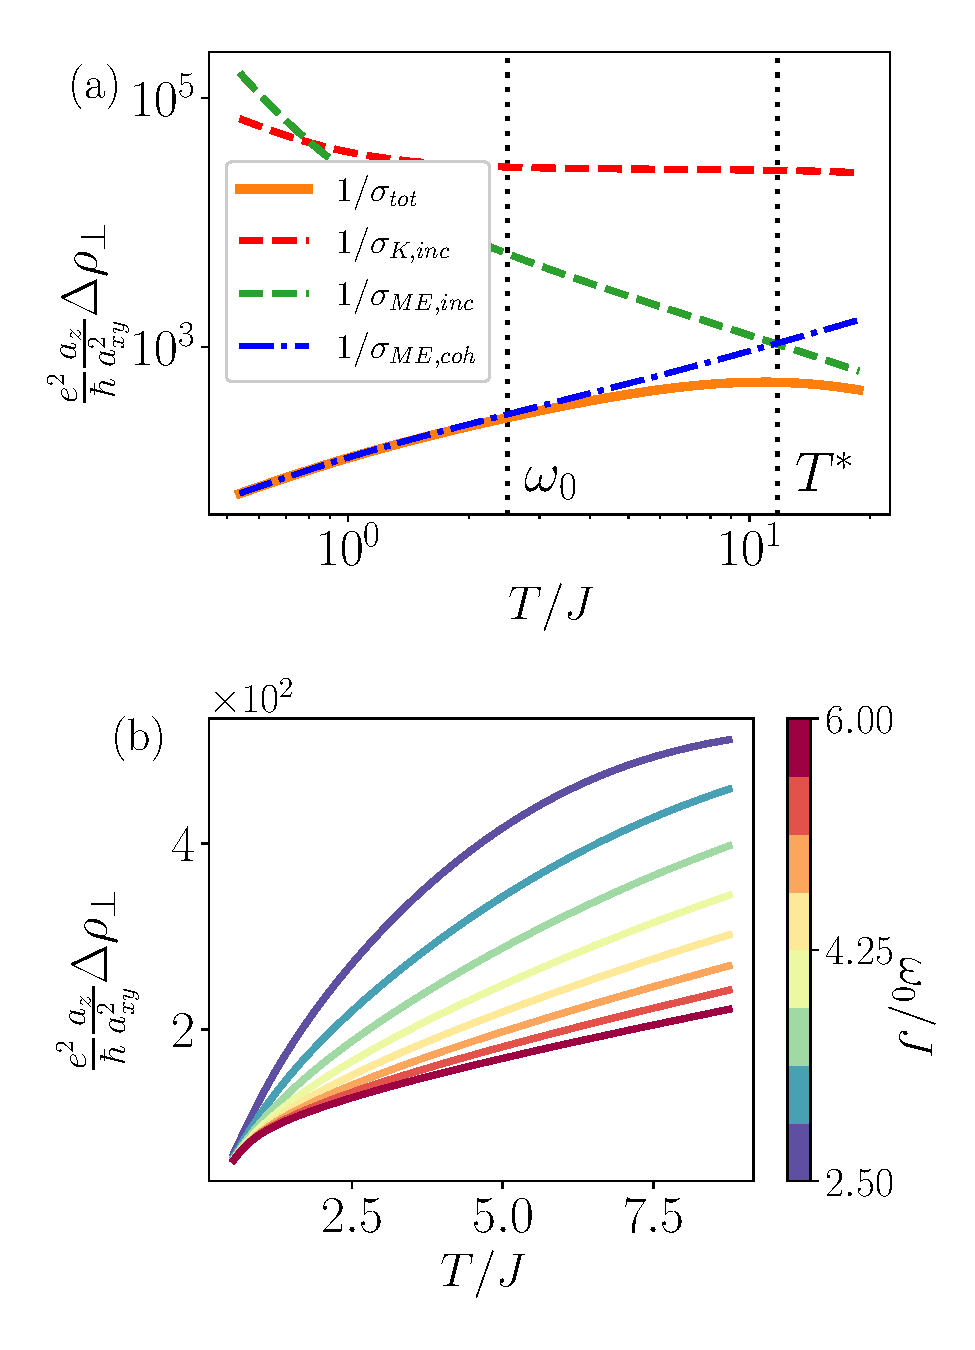
\includegraphics[width=0.45\textwidth]{out-of-plane.pdf} 
\caption{c-axis transport: (a) different contributions to the c-axis resistivity for a soft phonon frequency $\omega_0 =2.5 J_H$. Coherent transport dominates over a broad temperature regime but deviates from $T$ linearity at a temperature $T_*$ set by the electron velocity and the magnetoelastic coupling (see main text). The pure incoherent Kondo scattering is always shorted by other conducton channels. (b) Dependence of the c-axis resistivity on variations of the phonon frequency. As $\omega_0$ becomes softer the incoherent conductivty is enhanced and the coherent scattering increases making a saturation regime accessible at high temperatures. }
\label{fig:outofplane}
\end{figure}
%%%%%%%%%%%%%%%%

To calculate the conductivity we compute the current-current correlation for the total current $\bm{J}=\sum_{i}\bm{J}^{i}$. Since we work perturbatively in the Kondo and EME couplings, as well as in the out-of-plane hopping $t_{pp}$, the cross correlations between different current operators are subleading and we obtain 
\beq
\sigma^{c} &=& \sigma_{\text{inc}}+\sigma_{\text{coh}}\\
\sigma^{c}_{\text{inc}}&=& \lim_{\omega\rightarrow0}\lim_{\bm{q}\rightarrow0}\sum_{i=1,2}\frac{-1}{\beta V}\langle J^{i}_{z}(\tilde{q})J^{i}_{z}(-\tilde{q}) \rangle\\
\sigma^{c}_{\text{coh}}&=& 4 e^2 t_{pp}^2 a_z^2 \nu_0 \langle \tau_{\rm{tr}} \sin^2 k_z a_z  \rangle
\label{eqn:conducts_caxis}
\eeq

where $\langle \cdot \rangle $ denotes the momentum average over the Fermi surface, and $\nu_0$ is the density of states at the Fermi level. The behavior of each individual contribution to the conductivity is shown in Fig.~\ref{fig:outofplane}(a). Here we see that the incoherent contribution from the Kondo current $\bm{J}^1$ to the resistivity decreases with increasing $T$
and then saturates at a scale set by $J_{\rm H}$. In contrast the contribution of the EME current $\bm{J}^2$ to the resistivity continues to decrease with temperature with $\rho_{\text{inc, EME}}\sim T^{-1}$. At the same time the coherent contribution rises with temperature $\rho_{\text{coh}}\sim T$. We then obtain the total resistivity from parallel addition of each individual conduction channel. Interestingly, we note that there is a crossover temperature scale $T_*$ at which the incoherent and coherent resistivities coincide. At this scale, we expect resistivity saturation. At asymptotically high temperatures, there is an eventual change of trend where the resistivity decreases as a function of temperature as a consequence of incoherent processes. 

To estimate the scale at which this crossover occurs, we simply equate the high temperature limits of $\sigma^c_{\text{inc}}$ and $\sigma^c_{\text{coh}}$. Since the incoherent conductivity is dominated by the EME current correlations, we can approximate at high temperatures:
\beq
\sigma^c_{\text{inc}}\sim \left(\frac{a_{z}}{a_{xy}^{2}}\frac{e^{2}}{\hbar}\right)\lambda_{\rm{EME}}\nu_{0}T
\label{eqn:hight_inch}
\eeq
In the same regime, the coherent contribution to the conductivity can be well approximated by:
\beq
\sigma^c_{\text{coh}} \sim  \left(\frac{a_{z}}{a_{xy}^{2}}\frac{e^{2}}{\hbar}\right)\frac{t_{pp}^{2}\nu_{0}}{(\lambda_{\rm{EME}}+\lambda_{\rm{el-ph}}) k_{B}T}.
\label{eqn:hight_coh}
\eeq
Equating these two conductivities and estimating $v_z\sim t_{pp} a_z /\hbar$ we get the crossover temperature 
\begin{equation}
    T_*\sim\frac{v_z G_z}{\sqrt{\lambda_{\rm{EME}}(\lambda_{\rm{EME}}+\lambda_{\rm{el-ph}})} },
    \label{eqn:tstarscale}
\end{equation}
with $G_z=2\pi \hbar /a_z$. Note that the dependence on the density of states is now hidden in $\lambda_{\rm{EME}}$, which also depends on the frequency of the mode that mediates the EME interaction.

We now analyze the effect of pressure on the $c$-axis resistivity.
 Specifically, applying compressive strain along the $c$ direction introduces changes in the lattice constants, the hopping integrals, the Kondo coupling, and the phonon frequency. The expectation is that the phonon frequencies and lattice constants change algebraically while $J_{\rm{K}}$ and $t_{pp}$ change exponentially, so we focus on the latter in what follows. Additionally, we have $J_{\rm{K}} \propto t_{cp}^2/U,$ with $t_{cp}$ setting the scale of the hybridzation between Cr and Pd layers.  Consider the case where $t_{cp}^2$ has an exponential dependence on $a_z$ similar to that of $t_{pp}$. This could happen, for instance, if the inter-layer hopping is controlled by virtual tunneling via the Cr layers, then $t_{pp}$ is also proportional to $t_{cp}^2/U$. As a consequence, $J_{\rm{K}}$ increases at the same rate as $t_{pp}$ when pressure is applied along the $c-$axis. This entails that upon applying pressure, $\sigma^{c}_{\rm inc}$ grows since the overall scale of the incoherent current increased. At the same time, $\sigma^{c}_{\rm{coh}}$  increases since the increase in the $c-$axis velocity is matched by the increase of the scattering rate with decreasing $a_z$ for the Kondo and EME contributions, but not for the el--ph contribution. 

 
These changes to the resistivity also have an effect on the crossover scale $T_*$. With the scaling of the different hopping parameters, we find that $\lambda_{\rm EME}$ scales with $c$-axis pressure in the same way as $v_z^2$. Following Eqn.~\ref{eqn:tstarscale},  the crossover temperature $T_*$ is expected to decrease with increasing pressure. As such, deviations from $T$-linearity in the resistivity are expected to occur at lower temperatures when pressure is applied.   


\section{Incoherent contribution to the $c$-axis resistivity} \label{appendix_caxis_inc}


To evaluate the incoherent contribution to the conductivity we start
by Fourier transforming the current operators that are associated
with the Kondo and EME assisted hoppings between Pd layers.
These current operators are given by 
\begin{equation}
J^{1}_{z}\left(\omega_{n}\right)=\frac{1}{\sqrt{N\beta}}\sum_{\begin{array}{c}
\boldsymbol{k}\boldsymbol{k}'\alpha\beta\\
i\nu_{l},i\nu_{n}
\end{array}}f\left(\boldsymbol{k},\boldsymbol{k}'\right)p_{\boldsymbol{k}\alpha}^{\dagger}\left(i\nu_{l}\right)\left[\bm{S}_{\boldsymbol{k}-\boldsymbol{k}'}\left(i\nu_{l}-i\nu_{n}\right)\cdot\bm{\sigma}_{\alpha\beta}\right]p_{\boldsymbol{k}'\beta}\left(i\nu_{n}+i\omega_{n}\right)
\end{equation}
\begin{align}
J^{2}_{z}\left(\omega_{n}\right) & =\frac{1}{N\beta}\sum_{\begin{array}{c}
\boldsymbol{k}\boldsymbol{k}'\boldsymbol{q}\alpha\beta \ell \\
i\nu_{l},i\mu_{m},i\nu_{n}
\end{array}}\Lambda_{\ell}\left(\boldsymbol{k},\boldsymbol{k}'\right)\varphi^{(O)}_{\ell,\boldsymbol{k}-\boldsymbol{k}'-\boldsymbol{q}}\left(i\nu_{l}-i\mu_{m}-i\nu_{n}\right)p_{\boldsymbol{k}\alpha}^{\dagger}\left(i\nu_{l}\right)\left[\bm{S}_{\boldsymbol{q}}\left(i\mu_{m}\right)\cdot\bm{\sigma}_{\alpha\beta}\right]p_{\boldsymbol{k}'\beta}\left(i\nu_{n}+i\omega_{n}\right)
\end{align}
where the bare vertices are given by 
\begin{align}
f\left(\boldsymbol{k},\boldsymbol{k}'\right) & =J_{K}\left(\frac{2a_{z}}{\hbar}\right) \sin\left(k_{z}a_{z}+k_{z}'a_{z}\right),
\end{align}
and 
\begin{align}
\Lambda_{+}\left(\boldsymbol{k},\boldsymbol{k}'\right) & =\Lambda_{-}\left(\boldsymbol{k},\boldsymbol{k}'\right)=-\eta f\left(\boldsymbol{k},\boldsymbol{k}'\right)
\end{align}
we additionally parametrized the magnetoelastic interaction as $\tilde{\alpha}=-J_{k}\eta$
. Note that we have two phonon operators per local moment since there
are two bond streching modes, one that connects to the upper and one
that connects to the lower Pd layers. With these definitions, we proceed
to calculate the current-current correlation functions 
\begin{equation}
\Pi_{\boldsymbol{k}}^{zz}\left(i\omega_{n}\right)=\frac{-1}{\beta V}\sum_{i}\langle J_{z}^{i}(\tilde{q})J_{z}^{i}(-\tilde{q})\rangle=\Pi_{1}+\Pi_{2}
\end{equation}

There are two diagrams that contibute to leading order, these are
respectively:
\begin{fmffile}{diagram}
\begin{eqnarray}
\parbox{35mm}{\begin{fmfgraph}(100,100)\fmfleft{i} \fmfright{o}
   \fmf{dbl_dots}{i,v1} \fmf{dbl_dots}{v2,o}
   \fmf{dashes}{v1,v2}\fmffreeze
   \fmf{plain,left}{v1,v2,v1}
   \end{fmfgraph}} & = & \Pi_1  \\
   \parbox{35mm}{\begin{fmfgraph}(100,100)\fmfleft{i} \fmfright{o}
   \fmf{zigzag}{i,v1} \fmf{zigzag}{v2,o}
   \fmf{dashes,left=.5,tension=0.3}{v1,v2}\fmffreeze
   \fmf{boson,left=.5,tension=0.3}{v2,v1}\fmffreeze
   \fmf{plain,left}{v1,v2,v1}
   \end{fmfgraph}} & = & \Pi_2 
 \end{eqnarray}
 \end{fmffile}
where the dotted line corresponds to the $\boldsymbol{J}^{1}$ current,
the dashed line denotes the spin susceptibility, the zig-zag line is a $\boldsymbol{J}^{2}$
current, and the wiggly line is a phonon propagator. Note that there are no other phonon vertices since the interaction is diagonal in the phonon mode. If we allow for anharmonicities, further corrections to the $\Pi_2$ correlation function will contribute. 

The first diagram above amounts to the following expression:
\begin{equation}
\Pi_{\boldsymbol{k},1}^{zz}\left(i\omega_{n}\right)=\frac{1}{\beta V}\frac{1}{\beta N}\sum_{\boldsymbol{q}\boldsymbol{p}}\sum_{i\nu_{n}iz_{n}}\left|f\left(\boldsymbol{p}+\boldsymbol{q},\boldsymbol{k}+\boldsymbol{q}\right)\right|^{2}S\left(\boldsymbol{p},iz_{n}\right)\mathcal{G}\left(\boldsymbol{p}+\boldsymbol{q},i\nu_{n}+iz_{n}\right)\mathcal{G}\left(\boldsymbol{k}+\boldsymbol{q},i\omega_{n}+i\nu_{n}\right).
\end{equation}
We expect that in the high temperature limit vertex corrections
can be safely ignored in the perturbative regime when quasi-elastic
collisions dominate and there is no momentum structure to the scattering
potentials (since the spins are completely disordered). In this case, we proceed by performing the bosonic and fermionic Matsubara summations:
\begin{align}
\Pi_{\boldsymbol{k},1}^{zz}\left(i\omega_{n}\right) & =\frac{1}{V}\frac{1}{N}\sum_{\boldsymbol{q}\boldsymbol{p}}\left|f\left(\boldsymbol{p}+\boldsymbol{q},\boldsymbol{k}+\boldsymbol{q}\right)\right|^{2}\int\frac{d\epsilon}{\pi}\int\frac{d\nu}{\pi}\int\frac{dz}{\pi}\chi''\left(\boldsymbol{p},z\right)A\left(\boldsymbol{p}+\boldsymbol{q},\nu\right)A\left(\boldsymbol{k}+\boldsymbol{q},\epsilon\right) \nn \\
 & \ \ \ \ \ \ \ \ \ \ \ \ \ \ \ \ \ \ \ \ \times\left(\frac{n_{F}\left(\epsilon\right)-n_{F}\left(\nu-z\right)}{i\omega_{n}-\epsilon+\nu-z}\right)\left(n_{B}\left(z\right)+n_{F}\left(\nu\right)\right).
\end{align}
We see that overall the current correlation function is a convolution
of electron spectral functions with the spin susceptibility. Once
we perform analytic continuation and take the zero frequency limit,
we get 
\begin{equation}
\sigma_{11}^{c}=\frac{\hbar e^{2}}{VN}\sum_{\boldsymbol{q}\boldsymbol{p}}\left|f\left(p_{z},q_{z}\right)\right|^{2}\int\frac{d\epsilon}{\pi}\left[\int\frac{dz}{\pi}\chi''\left(\epsilon-z\right)A\left(\boldsymbol{p},z\right)\left(n_{B}\left(\epsilon-z\right)+n_{F}\left(-z\right)\right)\right]A\left(\boldsymbol{q},\epsilon\right)\left(-\frac{\partial n_{F}\left(\epsilon\right)}{\partial\epsilon}\right),
\end{equation}
where we already took the $\boldsymbol{k}\rightarrow0$ limit and
we used the local approximation on $\chi''$ to simplify the momentum
sums. Since the electron spectral functions satisfy $A\left(\boldsymbol{p},\omega\right)\approx A\left(\left(p_{x},p_{y}\right),\omega\right)$
we can pull the momentum sums over $q_{x,y}$ and $p_{x,y}$ past
the bare vertex, and to leading order we have 
\begin{equation}
\sigma_{11}^{c}=\frac{2a_{z}}{a_{pl}^{2}}\hbar e^{2}\int\frac{dp_{z}}{2\pi}\frac{dq_{z}}{2\pi}\left|f\left(p_{z},q_{z}\right)\right|^{2}\int\frac{d\epsilon}{\pi}\left[\int\frac{dz}{\pi}\chi''\left(\epsilon-z\right)\rho\left(z\right)\left(n_{B}\left(\epsilon-z\right)+n_{F}\left(-z\right)\right)\right]\rho\left(\epsilon\right)\left(-\frac{\partial n_{F}\left(\epsilon\right)}{\partial\epsilon}\right)
\end{equation}
using 
\[
\sigma_{11}^{c}=\left(\frac{2a_{z}}{a_{pl}^{2}}\frac{e^{2}}{\hbar}\right)J_{K}^{2}\int\frac{d\epsilon}{\pi}\rho\left(\epsilon\right)\left(-\frac{\partial n_{F}\left(\epsilon\right)}{\partial\epsilon}\right)\int\frac{dz}{\pi}\rho\left(\epsilon-z\right)\chi''\left(z\right)\left(n_{B}\left(z\right)+n_{F}\left(z-\epsilon\right)\right).
\]
To evaluate this integral we use the density of states evaluated from
the dispersion in the low energy theory of \cite{sunko_probing_2020}.

Now we focus on the EME current correlation functions
\[
\Pi_{\boldsymbol{q},2}^{zz}\left(i\omega_{n}\right)=-\frac{1}{\beta^{3}VN^{2}}\sum_{\begin{array}{c}
\boldsymbol{k}'\boldsymbol{k}\boldsymbol{p}\\
ik_{n}'ik_{n}ip_{n}\\
\ell
\end{array}}\left|\Lambda_{\ell}\left(\boldsymbol{k},\boldsymbol{k}'+\boldsymbol{q}\right)\right|^{2}D\left(\boldsymbol{k}-\boldsymbol{k}'-\boldsymbol{p},ik_{n}-ip_{n}-ik_{n}'\right)S\left(\boldsymbol{p},ip_{n}\right)\mathcal{G}\left(\boldsymbol{k},ik_{n}\right)\mathcal{G}\left(\boldsymbol{k}'+\boldsymbol{q},ik_{n}'+iq_{n}\right).
\]
Note that $D$ is independent of $\ell$ assuming that the frequencies of the two EME modes per unit cell are roughly equal. This is a consequence of the fact that the mass and the frequency of the two optical modes for the outgoing bonds from a local moment in the Cr layer are the same. Once again we can perform all three Matsubara sums, we then perform analytic continuation and take the appropriate DC limit, which gives the following expression for the c-axis conductivity:
\begin{align}
\sigma_{22}^{c} & =-\frac{e^{2}}{VN}\sum_{\boldsymbol{q}\boldsymbol{k}\ell}\int\frac{d\epsilon}{\pi}\frac{d\mu}{\pi}\frac{dz}{\pi}\left|\Lambda_{\ell}\left(\boldsymbol{q},\boldsymbol{k}\right)\right|^{2}B\left(z\right)\chi''\left(\mu\right)A\left(\boldsymbol{q},\epsilon+z+\mu\right)A\left(\boldsymbol{k},\epsilon\right)\times \nn \\
 & \ \ \ \left[n_{B}\left(-z\right)-n_{B}\left(\mu\right)\right]\left[n_{B}\left(z+\mu\right)+n_{F}\left(\epsilon+z+\mu\right)\right]\left(-\frac{\partial n_{F}\left(\epsilon\right)}{\partial\epsilon}\right).
\end{align}
Note that we have assumed to be a dispersion-less Einstein mode, which simplifies the momentum integrations. Once again, in the quasi 2D limit, we can perform the momentum sums first, which approximately converts each factor of the spectral function into a density of states. Finally, we use the phonon spectral function to evaluate one of the frequency integrals, which gives the result: 
\begin{align}
\sigma_{22}^{c} & =\left(\frac{2a_{z}}{a_{pl}^{2}}\frac{e^{2}}{\hbar}\right)\left(\frac{\hbar\eta^{2}}{M\omega_{0}}\right)\left[2J_{K}\right]^{2}\text{csch}\left(\frac{\beta\omega_{0}}{2}\right)\int\frac{d\epsilon}{\pi}\frac{d\mu}{\pi}\rho\left(\epsilon\right)\cosh\left(\frac{\beta\epsilon}{2}\right)\left(-\frac{\partial n_{F}\left(\epsilon\right)}{\partial\epsilon}\right)\times \nn \\
 & S\left(\mu\right)\left[\rho\left(\epsilon+\omega_{0}+\mu\right)\text{sech}\left(\beta\frac{\epsilon+\mu+\omega_{0}}{2}\right)+\rho\left(\epsilon-\omega_{0}+\mu\right)\text{sech}\left(\beta\frac{\epsilon+\mu-\omega_{0}}{2}\right)\right]\left[\frac{\beta\mu}{2}\text{csch}\left(\frac{\beta\mu}{2}\right)\right].
\end{align}
Importantly, the expression above can be simplified in the limit $\beta \omega \rightarrow 0$. In this case, it is straightforward to check that $\sigma^c_{22}\propto T$. 

\section{In-plane resistivity with acoustic phonons}
\label{appendix_acoustic}


In this section, we consider the contribution to the in-plane resistivity due to the EME term enabled scattering off acoustic phonons. A well-defined (i.e., parametrically large) $T^2$-scaling regime for $1/\tau_{\rm EME}$ exists provided $J_{\rm H}\ll \widetilde{T}_{\rm BG}$. We focus on temperatures, $J_{\rm H}\ll T \ll \widetilde{T}_{\rm BG}$, with $\widetilde{T}_{\rm BG} = 2\widetilde{c}k_F$ being the EME Bloch-Gr\"uneisen (BG) temperature. In this regime, we only consider the effects of quasi-elastic scattering off the spins which have approximately local correlations, such that the spin structure factor can be approximated as a constant in momentum space \textit{and} a delta function in frequency space \cite{mcroberts2022intermediatescale}. In other words, phonons provide a source of inelastic scattering while the uncorrelated spins make this scattering isotropic. This is in contrast to the conventional electron-phonon interaction, where the scattering is mainly small-angle up to the BG temperature. A schematic for the scattering processes is shown in Fig.~\ref{fig:eme_acoustic_phonon}.


\begin{figure}[h]
\centering
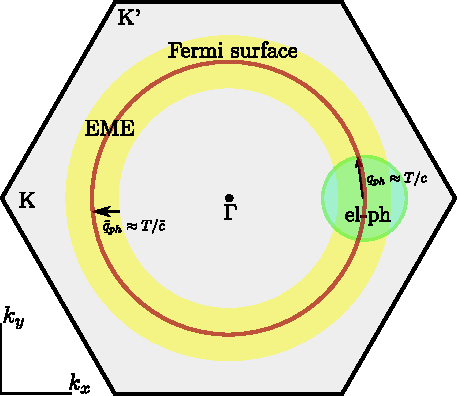
\includegraphics[width=0.45\textwidth]{BZ1_scattering1_disordered.pdf} 
\caption{A typical scattering event due to the EME interaction in the local approximation, wherethe spin structure factor is assumed to be featureless, i.e., $S(\omega,\boldsymbol{q}) \approx \rm{const} \times \delta(\omega)$. Starting from $\boldsymbol{k}$ (center of green circle) on the Fermi surface (red circle), the local-moments scatter the momentum uniformly throughout the Brillioun zone via the EME term, such that the annulus (yellow) of phonon modes with momenta $\widetilde{q}_{ph} \leq T/\widetilde{c}$ efficiently scatters electrons isotropically on the Fermi surface. In contrast, the conventional el-ph interaction efficiently scatters electrons to a region enclosed by a sphere of radius $q_{ph} \approx T/c$, as shown in the green circle, such that scattering is mainly small-angle up to $\widetilde{T}_{\rm BG}$. 
}
\label{fig:eme_acoustic_phonon}
\end{figure}

 
Let us first recall the contribution to the electron-phonon transport scattering time \cite{Allen1993,sadovskii_diagrammatics_2019} within Boltzmann theory (equivalent to Eq.~\eqref{tr_time}), 
\begin{equation}
    \frac{1}{\tau_{\text{el-ph}}}=\frac{4\pi}{\beta}\int_{\Omega}\frac{d\Omega}{\Omega}\alpha^{2}F_{\text{tr}}\left(\Omega\right)\mathcal{K}\left(\beta\Omega\right).
\end{equation}
In the Debye approximation for an acoustic mode in 2D, where $\alpha^{2}F_{\text{tr}}\left(\Omega\right)\approx \lambda_{\text{el-ph}} (3/2)\left(\Omega/\Omega_{D}\right)^{3}\theta\left(\Omega_{D}-\Omega\right)$, there is a factor of $\left(\Omega/\Omega_{D}\right)^{2}$ in the el-ph matrix element due to the weighting of small-angle scattering: $1-\cos\left( \theta_{\boldsymbol{k},\boldsymbol{k'}}\right) \sim q^2 \sim \Omega^2$, where $\boldsymbol{k},\boldsymbol{k'}$ are points on the Fermi surface and $\boldsymbol{q}$ is the phonon wavevector, see e.g., \cite{Ziman_2001}. In contrast, this weighting is absent in the isotropic EME transport time for reasons highlighted above, which can therefore be approximated as 
\begin{equation}
    \frac{1}{\tau_{\text{EME}}}=\frac{4\pi}{\beta}\int_{\Omega}\frac{d\Omega}{\Omega}\alpha^{2}F_{\text{EME}}\left(\Omega\right)\mathcal{K}\left(\beta\Omega\right),
\end{equation}
where $\alpha^{2}F_{\text{\text{EME}}}\left(\Omega\right)\approx\frac{1}{2}\lambda_{\text{EME}}\left(\Omega/\widetilde{\Omega}_{\text{BG}}\right)\theta\left(\widetilde{\Omega}_{\text{BG}}-\Omega\right)$ (note that $\widetilde{\Omega}_{\rm BG} = \widetilde{T}_{\rm BG}$) and $\mathcal{K}$ defined by Eq.~\eqref{def_of_K}. Here we have assumed the BG temperature, rather than the Debye temperature, to be the relevant scale for transport. As described in Fig.~\ref{fig:eme_acoustic_phonon}, the dominant scattering is from thermally excited phonons, which can be seen here by the exponential suppression of $\mathcal{K}(x>1)$. Scattering in this regime if therefore quasi-elastic. In total, we obtain that
\begin{equation}
    \frac{1}{\tau_{\text{EME}}}\approx2\pi\lambda_{\text{EME}}\frac{T^{2}}{\widetilde{T}_{\text{BG}}}, \quad J_{\rm H} \ll T \ll \widetilde{T}_{\rm BG},
\end{equation}
while for $T\gtrsim \widetilde{T}_{\rm BG}$, $1/\tau_{\text{EME}}\approx2\pi\lambda_{\text{EME}}T$, as discussed earlier.


\end{widetext}

\bibliography{refs.bib}

\end{document}